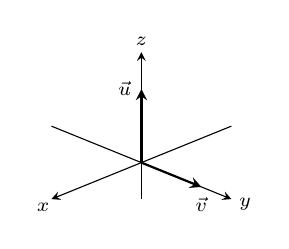
\begin{tikzpicture}[>=stealth]
\begin{axis}%
[width=175pt,tick label style={font=\scriptsize},axis on top,
			axis lines=center,
			view={135}{35},
			name=myplot,
			xtick=\empty,
			ytick=\empty,
			ztick=\empty,
			ymin=-1.5,ymax=1.5,
			xmin=-1.5,xmax=1.5,
			zmin=-0.5, zmax=1.5,
			every axis x label/.style={at={(axis cs:\pgfkeysvalueof{/pgfplots/xmax},0,0)},xshift=-3pt,yshift=-3pt},
				xlabel={\scriptsize $x$},
			every axis y label/.style={at={(axis cs:0,\pgfkeysvalueof{/pgfplots/ymax},0)},xshift=5pt,yshift=-2pt},
				ylabel={\scriptsize $y$},
				every axis z label/.style={at={(axis cs:0,0,\pgfkeysvalueof{/pgfplots/zmax})},xshift=0pt,yshift=4pt},
				zlabel={\scriptsize $z$}
			]

\draw [thick,->,{\colorone}] (axis cs:0,0,0) -- (axis cs:0,0,1) node [black,left] {\scriptsize $\vec u$};
\draw [thick,->,{\colorone}] (axis cs:0,0,0) -- (axis cs:0,1,0) node [black,below] {\scriptsize $\vec v$};

%\draw [thick,->,{\colorone}] (axis cs:0,0,0) -- (axis cs:0,1,1) node [black,above] {\scriptsize $\vec u+\vec v$};
%
%\draw [thick,->,{\colorone}] (axis cs:0,1,0) -- (axis cs:0,0,1) node [black,right,pos=.2] {\scriptsize $\vec u-\vec v$};

\end{axis}

\end{tikzpicture}











